\graphicspath{{images/tn-gp-sagit/drafts/}}

\chapter{Study IV: Gaussian Process Classification of Trigeminal Neuralgia using Merged Group Tractography}
\chaptermark{Study IV}
\label{section:study4}

\section{Abstract}
\textbf{Introduction:}  Imaging of trigmeinal neuralgia (TN) has demonstrated key diffusivity alterations in the trigeminal nerve but the difficulties of group tractography analysis have previously prevented us from assessing the entire trigeminal pathway. We apply fully-automated group white-matter tractography to now image the trigeminal sensory pathway, and Gaussian Process (GP) classification to pinpoint key white-matter diffusivity changes that maximally differentiate TN in patients and healthy controls. 

\textbf{Methods:} We used SAGIT based group merged tractography for 36 sex-matched TN patients (right-sided pain) and 36 controls, examining the following white matter pathways: trigeminal nerve (CN V), pontine decussation, and thalamocortical fibers. GP classifiers were trained by scrolling a moving window over CN V and S1 tractography centroids. FA, GFA, RD, AD, and MD metrics were evaluated for both groups, analysing TN vs. Control and affected vs. unaffected groups. Classifiers that performed at greater-or-equal-to 70\% accuracy were accepted.

\textbf{Results:} Both affected and unaffected trigeminal nerves in TN patients can be differentiated with 80\% accuracy from controls. Affected CN V FA segments that are differentiated from trons have more overlap towards the distal segments in the cistern and gangion, whereas unaffected CN V segment overlaps extend more towards the brainstem. The bilateral middle segment of S1 can be differentiated from controls. Where the affected S1 RD classifier achieved higher accuracy of 87\%.

\textbf{Conclusions:} We  demonstrate the first instance of group-wise merged tractography analysis of TN vs. control and TN white-matter machine learning classification using GP. The method reproduced previous findings with finer-grained regional specificity. The study also revealed specific diffusivity changes in TPT and S1 white matter pathways.

\section{Introduction}
\subsubsection{Trigeminal Neuralgia}
Trigeminal neuralgia (TN) is a debilitating facial neuropathic pain syndrome characterized by paroxysmal and shock-like pain in one or more dermatomes of the three trigeminal nerve (The fifth cranial nerve: CN V) branches. TN manifests most commonly as classic (also called idiopathic TN), or secondary to a range of neuropathology, including tumors such as meningiomas \cite{Cheng2008}, trigeminal schwannomas \cite{Miller2008}, neurocysticercosis \cite{Revuelta1995}, and most notably multiple-sclerosis (MS) \cite{Cruccu2009,VanderMeijs2002,Nick2012}. The pathophysiology of idiopathic TN is thought to be vascular compression at the root of the CN V nerve entry zone (NEZ) \cite{Linn2011,Love2001}, although idiopathic TN can also occur without evidence of vascular compression \cite{Lee2014}. We previously compared TN and MS-TN diffusivity differences in four segments of the CN V at the level of the pons \cite{Chen2016a}, and confirmed that brainstem CN V diffusivity is altered in MS-TN. 

The trigeminal sensory system involves both the discriminative touch and pain pathways. Anatomically, the discriminative pathway synapses onto the primary trigeminal sensory nucleus, and then projects to the contralateral VC thalamus and then to the S1 cortex. The nociceptive pathway synapses caudally onto the trigeminal spinal nucleus, decussates at the level of the medulla and spinal cord. The pathway merges with the discriminative sensory pathway and ascend as the contralateral trigeminal lemniscus, and also project to the contralateral VC thalamus. The pain pathway also projects to the medial nucleus of the thalamus, where it then project medially to the cingulate cortex. 

\subsubsection{Along-the-tract analysis}
White matter tractography is commonly used for anatomical visualization \cite{Chen2011b}, white matter segmentation \cite{Behrens2003a,Johansen-Berg2005}, and structural connectivity analysis \cite{Cao2013,Wiech2014}. Obtaining diffusivity metrics from tractography involves converting streamline bundles into a volumetric spatial mask, followed by measurement of the mean metric from all or parts of the masked voxels \cite{Concha2005,Fitzsimmons2009}. However this approach discards the orientation information in the streamlines. The simplest form of spatial masking is to identify voxels where at least one streamline has passed through it, which often results in identifying voxels with minimal streamline pass-throughs. This is potentially problematic when considering that an average 3-Tesla HARDI DWI acquisition has a voxel dimension of 2 to 3 mm. In white matter structures such as CN V as well as other small pathways, the structure diameter may be no more than 3mm, and therefore the naive spatial masking approach would result in severe partial volumes that will confound the result. 

In this light, it must be considered that a tractography streamline propagation algorithm involves all or parts of the following stages: 1) subsampling of an initial region for seeding \cite{Basser2002,Cote2012}; 2) identifying a propagation direction, based on previously traversed paths \cite{Malcolm2010,Qazi2009,Tournier2010}; 3) smoothing of the traversed paths for output \cite{Tuch2000d}. It is reasonable to consider these algorithms to be an interpolated subsampling scheme of the DWI volume that takes the diffusion-based orientation into account. Therefore, it would be desirable to directly make use of the tractography streamlines for data measurement. 

Along-the-tract analysis has been investigated by various authors \cite{Colby2012,ODonnell2009,Wang2015,Yeatman2012}. In these approaches, the bundles were selectively filtered from global tractography \cite{Wang2015,Yeatman2012}, and limited to major white matter bundles such as the corpus callosum, corticospinal tract, longitudinal fasciculus, arcuate fasciculus, and uncinate. The measures were pooled onto tract centroid in each individual subjects, and then aggregated at the group level. The global tractography approach is unintuitive for anatomy-specific tasks such as neurosurgical planning, where the anatomy of interest is clear. A more focused ROI based delineation approach is therefore preferred in these circumstances.

It is important to note that streamline clustering and centroid identification can be considered as independent tasks. Some clustering methods do not provide a best-representative streamline centroid. Centroid identification involves resampling the streamlines into an identical number of points, and then identifying point correspondences via different distance measures. For these approaches, streamlines require similar length, and an assumption that the start and end of the streamlines across subjects is consistent. However, pathological brain tissue may negatively affect tractography delineation. Therefore the geometry assumptions of such approaches may not be satisfied when studying patient populations. Running time and memory constraints also need to be taken into consideration when applying such algorithms at a group level. We have adopted QuickBundles since it is a practical method of tract clustering and centroid identification with linear running time to obtain S1 streamline centroids. \cite{Garyfallidis2012}

The principal advantage of a streamline-based approach is that we can preserve the fiber orientations. White matter metrics in 3D space can then be projected to a lower dimensional centroid for detailed analysis. We have developed the Selective Automated Group Integrated Tractography (SAGIT) framework (Chen et al., 2016) to automate group-wise tractography delineation, which ensures consistent region-of-interest projection, tractography seeding sampling scheme, and tractography parameter tuning. We then merge the tracts into a template space using non-linear deformations, and  perform tractography centroid identification and statistics at the merged group level to ensure anatomical consistency. 

\subsubsection{Gaussian Process}
The breakthrough results of deep convolutional neural networks in computer vision \cite{Krizhevsky2012} have sparked the interest of deploying similar systems for medical imaging diagnosis \cite{Greenspan2016}. However, one disadvantage of deep neural networks is in its inability to quantify uncertainty and provide interpretable models. Model interpretability is a fundamental requirement for machine learning in medicine, and therefore there is renewed interest in bayesian-based models like Gaussian Process (GP) \cite{gal2016dropout}.

Gaussian Process is defined \cite{rasmussen2006gaussian} as a collection of random variables, any finite number of which have a joint Gaussian distribution. 
It is a distribution that is defined by a mean function $m(x)$ and covariance function $k(x,x') $ where
\begin{equation}
	\begin{split}
		m(x) &= \mathbb{E}[f(x)], \\
		k(x,x') &= \mathbb{E}[(f(x)-m(x)(f(x')-m(x'))],
	\end{split}
\end{equation}
And the Gaussain processed is defined as
\begin{equation}
f(x) \sim GP(m(x), k(x, x')) 
\end{equation}

The covariance function is termed called kernel function. The radial-basis function kernel (RBF kernel) is widely used in machine learning tasks. GP has previously been explored in neuroimaging for tractography clustering \cite{Wassermann2010} and it is particularly well suited for continuous data streams, such as tractography streamlines.

In all previous TN studies, placements of measurement region-of-interests in the CN V were pre-planned and manually placed by researchers. Manual tractography generation with manual ROI placements was a roadblock in performing more indepth group-wise tractography examination of the trigeminal pathways. We had developed and validated the SAGIT tractography framework to allow automated group tractography \cite{Chen2016}. In this study we further expand the study to A) analyze the CN V differences between TN and healthy controls across the entire nerve using along-the-track and machine-learning methods to auto-discover key regions-of-interest; B) extend the examined regions to include trigeminopontothalamic (TPT) and thalamocortical (S1) white matter pathways as part of the trigeminal sensory pathways.

\section{Methods}
\subsubsection{Acquisitions}
We studied 36 patients with classic TN (28 females, 8 males; age 60.1$\pm$16 years; right sided pain), and 36 healthy controls (28 females, 8 males, age 42.7$\pm$12 years).  All patients underwent non-invasive Gamma Knife radiosurgery, with imaging prior and six months post treatment. MRI acquisitions including T1 fast-spoiled gradient echo (FSPGR) and diffusion weighted image (DWI) acquisitions. T1 scans were acquired with 1mm slice thickness, in-plane resolution of 0.9375x0.9375mm, slice spacing=1 mm, TE=5.052 ms, TR=11.956 ms, flip angle=20 deg, FOV=240 mm, and matrix=256x256. DWI scans were acquired with 1 B0 scan, 60 gradient directions, 3mm slice thickness and an in-plane resolution of 0.9375x0.9375 mm, b0=1000 s/mm2, TE=88.6 ms, TR=17000 ms, flip angle=90 deg, field of view (FOV)=120 mm, and matrix=128x128.

\subsubsection{Preprocessing}
DWI images were motion/eddy-current corrected, with appropriate correction applied to the b-matrix \cite{Leemans2009}. Region of interests (ROI) for tractography seeding were manually created on a normalized template brain from 42 healthy brains \cite{Chen2016}. The normalized brain template was created using Anatomical Normalization Tools \cite{Avants2010,Avants2011}. We deployed selective automatic group integrated tractography (SAGIT) framework \cite{Chen2016} to automate preprocessing, registration, and tract generation. The SAGIT processing steps are as follows: T1 anatomical images were processed using FreeSurfer \cite{Fischl2004} for cortical and subcortical segmentations. The T1 images for all the subjects were registered to the template using symmetric diffeomorphic registration (SDR) \cite{Avants2008b}. Each individual DWI was registered to their T1 image with SDR, using mean DWI image for DWI-T1 co-registration. Freesurfer segmentation maps were first affine transformed from the Freesurfer space to the T1 space using FMRIB's Linear Image Registration Tool (FLIRT) \cite{Jenkinson2001,Jenkinson2002}, and then transformed using SDR transforms to the individual DWI space for selective ROI generation with SAGIT.

\subsubsection{Tractography}
ROIs were defined on the template image to delineate the following bilateral structures: 1) CN V (ROI placed at cistern nerve root; excludes regions of cerebellum grey matter and pontine cerebellar peduncles); 2) trigeminothalamic pontine decussation (TPT) (ROIs placed at trigeminal nucleus (TGN); the fibers must traverse pontine decussation towards contralateral VC thalamus; pathway must exclude ipsilateral thalamus, cerebellar grey matter, pons, and contra-lateral S1 ); 3) thalamocortical S1 pathway (ROIs placed at VC thalamus; pathway must traverse the ipsilateral S1 white-matter boundary; it must exclude the brainstem).  

We used constrained spherical deconvolutional tractography (CST) \cite{Tournier2012b} to delineate the three defined anatomical regions. Deterministic and probabilistic streamline algorithms were used to delineate different regions, based on findings in the SAGIT study \cite{Chen2016}. Deterministic CST was applied to delineate CN V and S1 anatomy, while probabilistic (iFOD2) CST \cite{Jeurissen2011b,Tournier2010} was applied to delineate TPT anatomy. The parameters for each were as follows: Deterministic CST was performed with step size = 0.3mm, angle threshold = 45$\deg$, streamline count=200, minimal length = 5 mm, initial cut-off = 0.1, cut-off = 0.1, and with 4th-order Runge-Kutta integration. Probabilistic tractography for S1 projection was performed with step size = 5mm, angle threshold = 45$\deg$, streamline count = 300, max number of stream generation = 1 million, minimal length = 10 mm, maximum lengh = 80 mm, initial cut-off = 0.15, cut-off = 0.15. Probabilistic tractography for TPT project was performed with step size = 1mm, and streamline count = 2000, and maximal length = 60 mm. Tractography was first performed in the native DWI space for each subject.  FA, AD, RD, MD, and GFA were embedded into the native tractography models by sampling the corresponding images maps using the points of the tractography geometry with tri-linear interpolation.

\subsubsection{Merged Tractography}
All tractography delineations of the same anatomy across all the subjects and groups were merged into a single tractography file for analysis. A software library\footnote{https://github.com/sinkpoint/fascicle} is created by the author to facilitate this process, the steps are as follows: The individual tract files were converted into a SQLite relational database \cite{owens2010sqlite}, and  all points were exported and transformed by applying the subject DWI to T1, and T1 to template transforms using ANTS' applyTransformToPoints command \cite{Avants2009}. The transformed points were then imported back into the  database, and a new template-space tractography model is exported using the transformed point-set, with all its original scalars and subject/group associations preserved. Finally, all template-space tractography models across all the subjects are merged into a single file. 

\subsubsection{Along-the-tract Analysis}
The merged tract was post-processed in 3D Slicer to remove erroneous streamlines that confounded measurement. Streamlines removed include remnant CN V streamlines that stray into the cerebellar peduncles or other non-TGN regions, and streamlines that are perpendicular to the nerve in the cisternal space that appear to be partial delineation of vessels or noise. TPT streamlines that did not decussate at the level of the pons, as well as fibers that stray into the contralateral TGN were removed. S1 streamlines that stray medially towards other regions such as the corpus callosum were also removed.

Tractography centroids, which were the average curve best fit the tract bundle, were identified on the merged tracts in template space. CN V centroids were manually defined using 3 control points. A Catmull-Rom spline \cite{DeRose1988} was then defined from these control points using the VTK software library \cite{Schroeder2005}, which resulted in a curve of length 38.91 mm. The spline is then resampled into 30 points that become the centroid definition with segment length of 1.3 mm. Nearest-neighbor point assignment was used to divide the merged tract into 30 cross sections along the centroids. Diffusion metrics from the points were aggregated for each of the cross-sections.  S1 centroids were defined using QuickBundles \cite{Garyfallidis2012} with distance threshold of 30, resulting in centroid length of 62.1 mm and segment length of 2.07 mm. 

\subsubsection{Gaussian Process Classification}

Diffusivity metrics of affected (right side) and unaffected CN V and S1 pathways were independently compared with those of controls, where control metrics were the average of both left and right sides. The affected and unaffected sides in TN patients were also compared with each other. 
Age was regressed out by using the residuals of the linear regression model from the controls group. The diffusion values were subsequently normalized to zero mean with ranges $[-1, 1]$ for model training. 
Gaussian Process (GP) classification was performed on CN V and S1 nerve segments to identify key segment differences. Multiple moving windows of length between 5 to 30 were used to constraint tract segments, and a Gaussian Process model was trained for each windowed segment. The entire machine learning process was performed using Scikit-learn machine learning software framework.
For each model, the subjects were split into train and validation sets using stratified 10-fold cross-validation. The GP model was initiated with Matern kernel (length scale = 1), and the model fitted using the training set. The validation set was used to measure prediction accuracy, and the mean accuracy of the 10-fold cross-validation was used to assess the windowed segment. Segments accuracy greater than 75\% were accepted, and the segment length with the greatest accuracy was then determined. 

\subsection{Results}
\subsubsection{Tractography}
Merged CN V delineations show anatomical consistency, and extended into the ipsilateral TGN. Changes in FA along the streamlines demonstrate clear differences between cistern and brainstem segments, suggesting good agreement in anatomical registration ( Figure \ref{fig:GPfigure1}). 
The TPT projections, when filtered strictly from the TGN to the ipsilateral VC thalamus region, showed distinct bundles of decussating pathways between left and right. The resulting pathway was not symmetrical, where the right TPT pathway diverts and envelopes the left (Figure \ref{fig:GPfigure2}).
S1 streamlines reliably extended into the face region of the S1 cortex (Figure \ref{fig:GPfigure3}). 

\begin{figure}[ht]
\centering
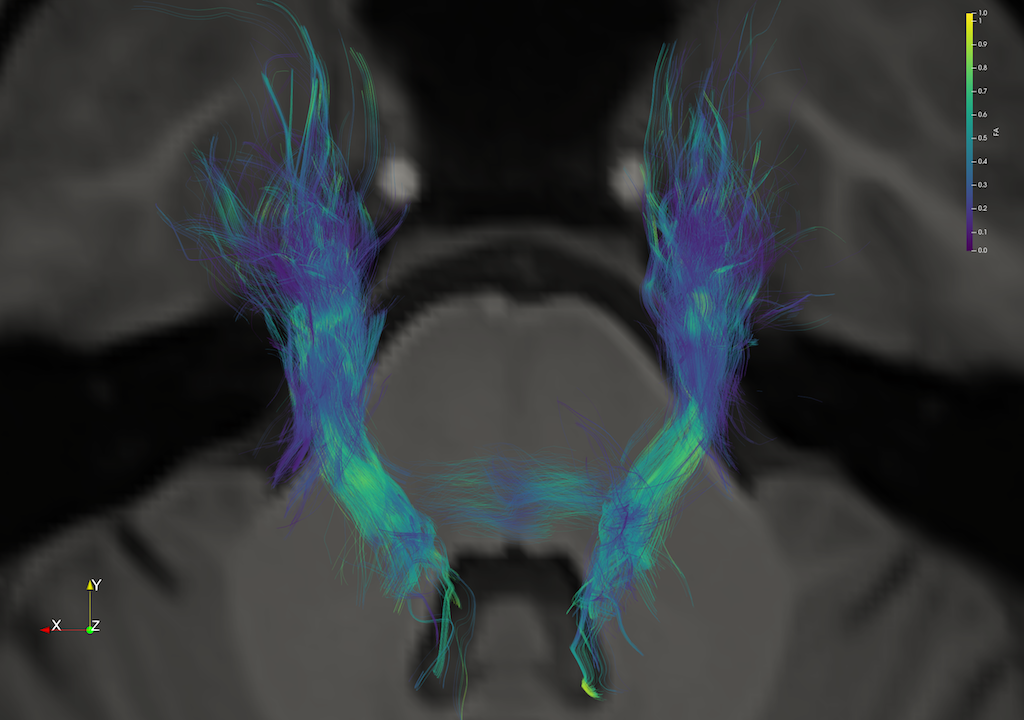
\includegraphics[width=\linewidth]{cnv-inferior-view.png}
\caption{Inferior view of the merged CN V delineations.}
\label{fig:GPfigure1}
\end{figure}

\begin{figure}[ht]
\centering
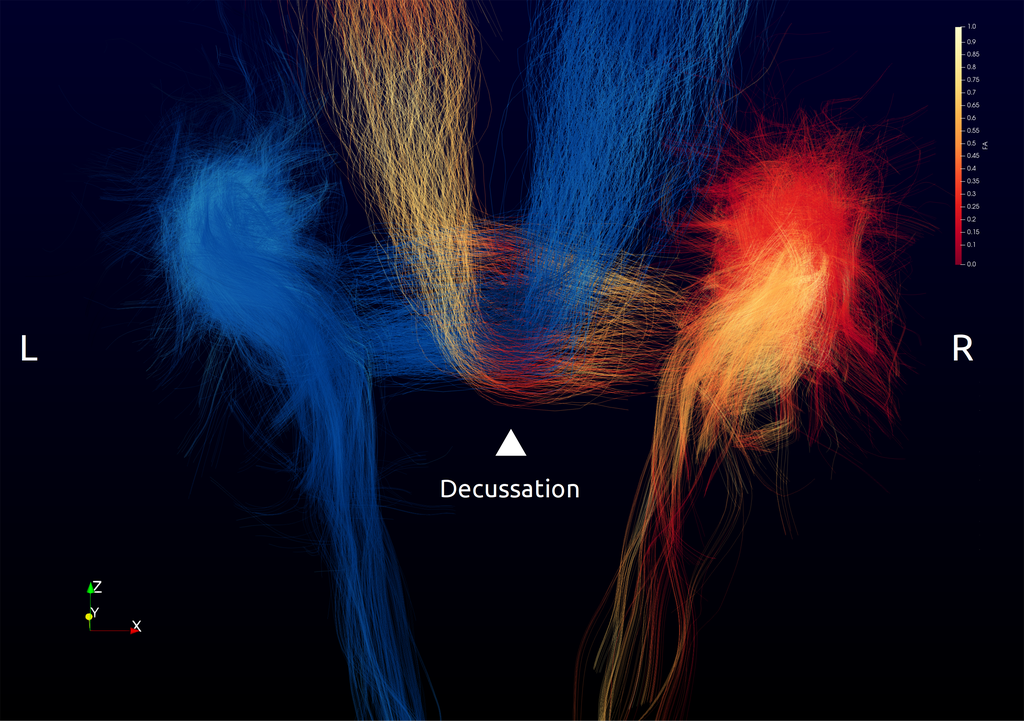
\includegraphics[width=\linewidth]{view-decussation.png}
\caption{Close up of the TPT decussation. Red: Right TPT; Blue: Left TPT. Note the Right TPT diverts around the left TPT bundle. }
\label{fig:GPfigure2}
\end{figure}

\begin{figure}[ht]
\centering
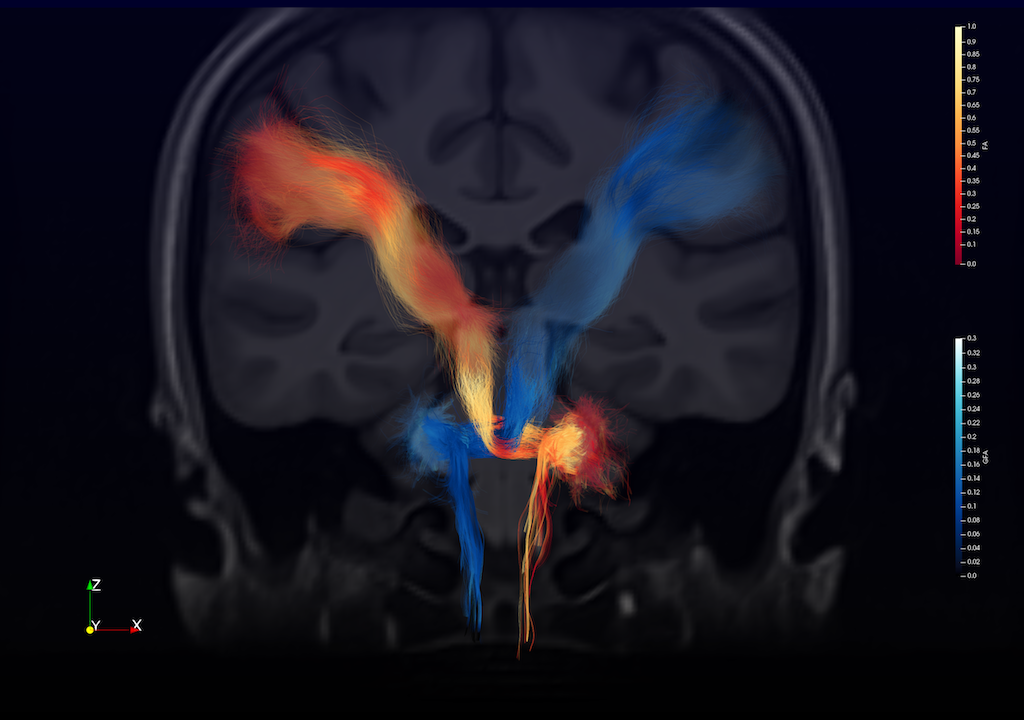
\includegraphics[width=\linewidth]{view-left-right.png}
\caption{The complete trigeminal discriminatory sensory pathway. }
\label{fig:GPfigure3}
\end{figure}

\subsubsection{Diffusivity Differences}
\paragraph{CN V}
Both sides were distinguished from controls with classifiers that achieve around 80\% accuracy (Figure \ref{fig:GPfigure4}). 
Classifiers on the right side have performance ranging from 76\% (GFA) to 86\% (FA) accuracy. The left classifiers achieved accuracy ranging from 79\% (MD) to 81\%(FA). The right side shows more overlap of segment ranges between positions 14--24, in the region of the cistern/gangion; while the left side shows segments that covers the entire the nerve, and extends to cover position 0--4 in the brainstem. Overall, the right side features extend further into the distal space, into the cistern and even the ganglion, while the left side extends more into the brainstem. FA consistently achieved the highest accuracy in both sides, with right FA at position 17--23 (cistern/ganglion) and left FA at 2--16 (brainstem/cister).
Comparing left/right, the FA classifier achieved 75\% accuracy, where its segments range from 11 to 19, which is the cisternal segment. The GFA classifier achieved 70\% accuracy in region 9--12. Demonstrating that affected-unaffected diffusivity differences are found in the cistern/REZ (Table \ref{table:CN V}).

\begin{figure}[ht]
\centering
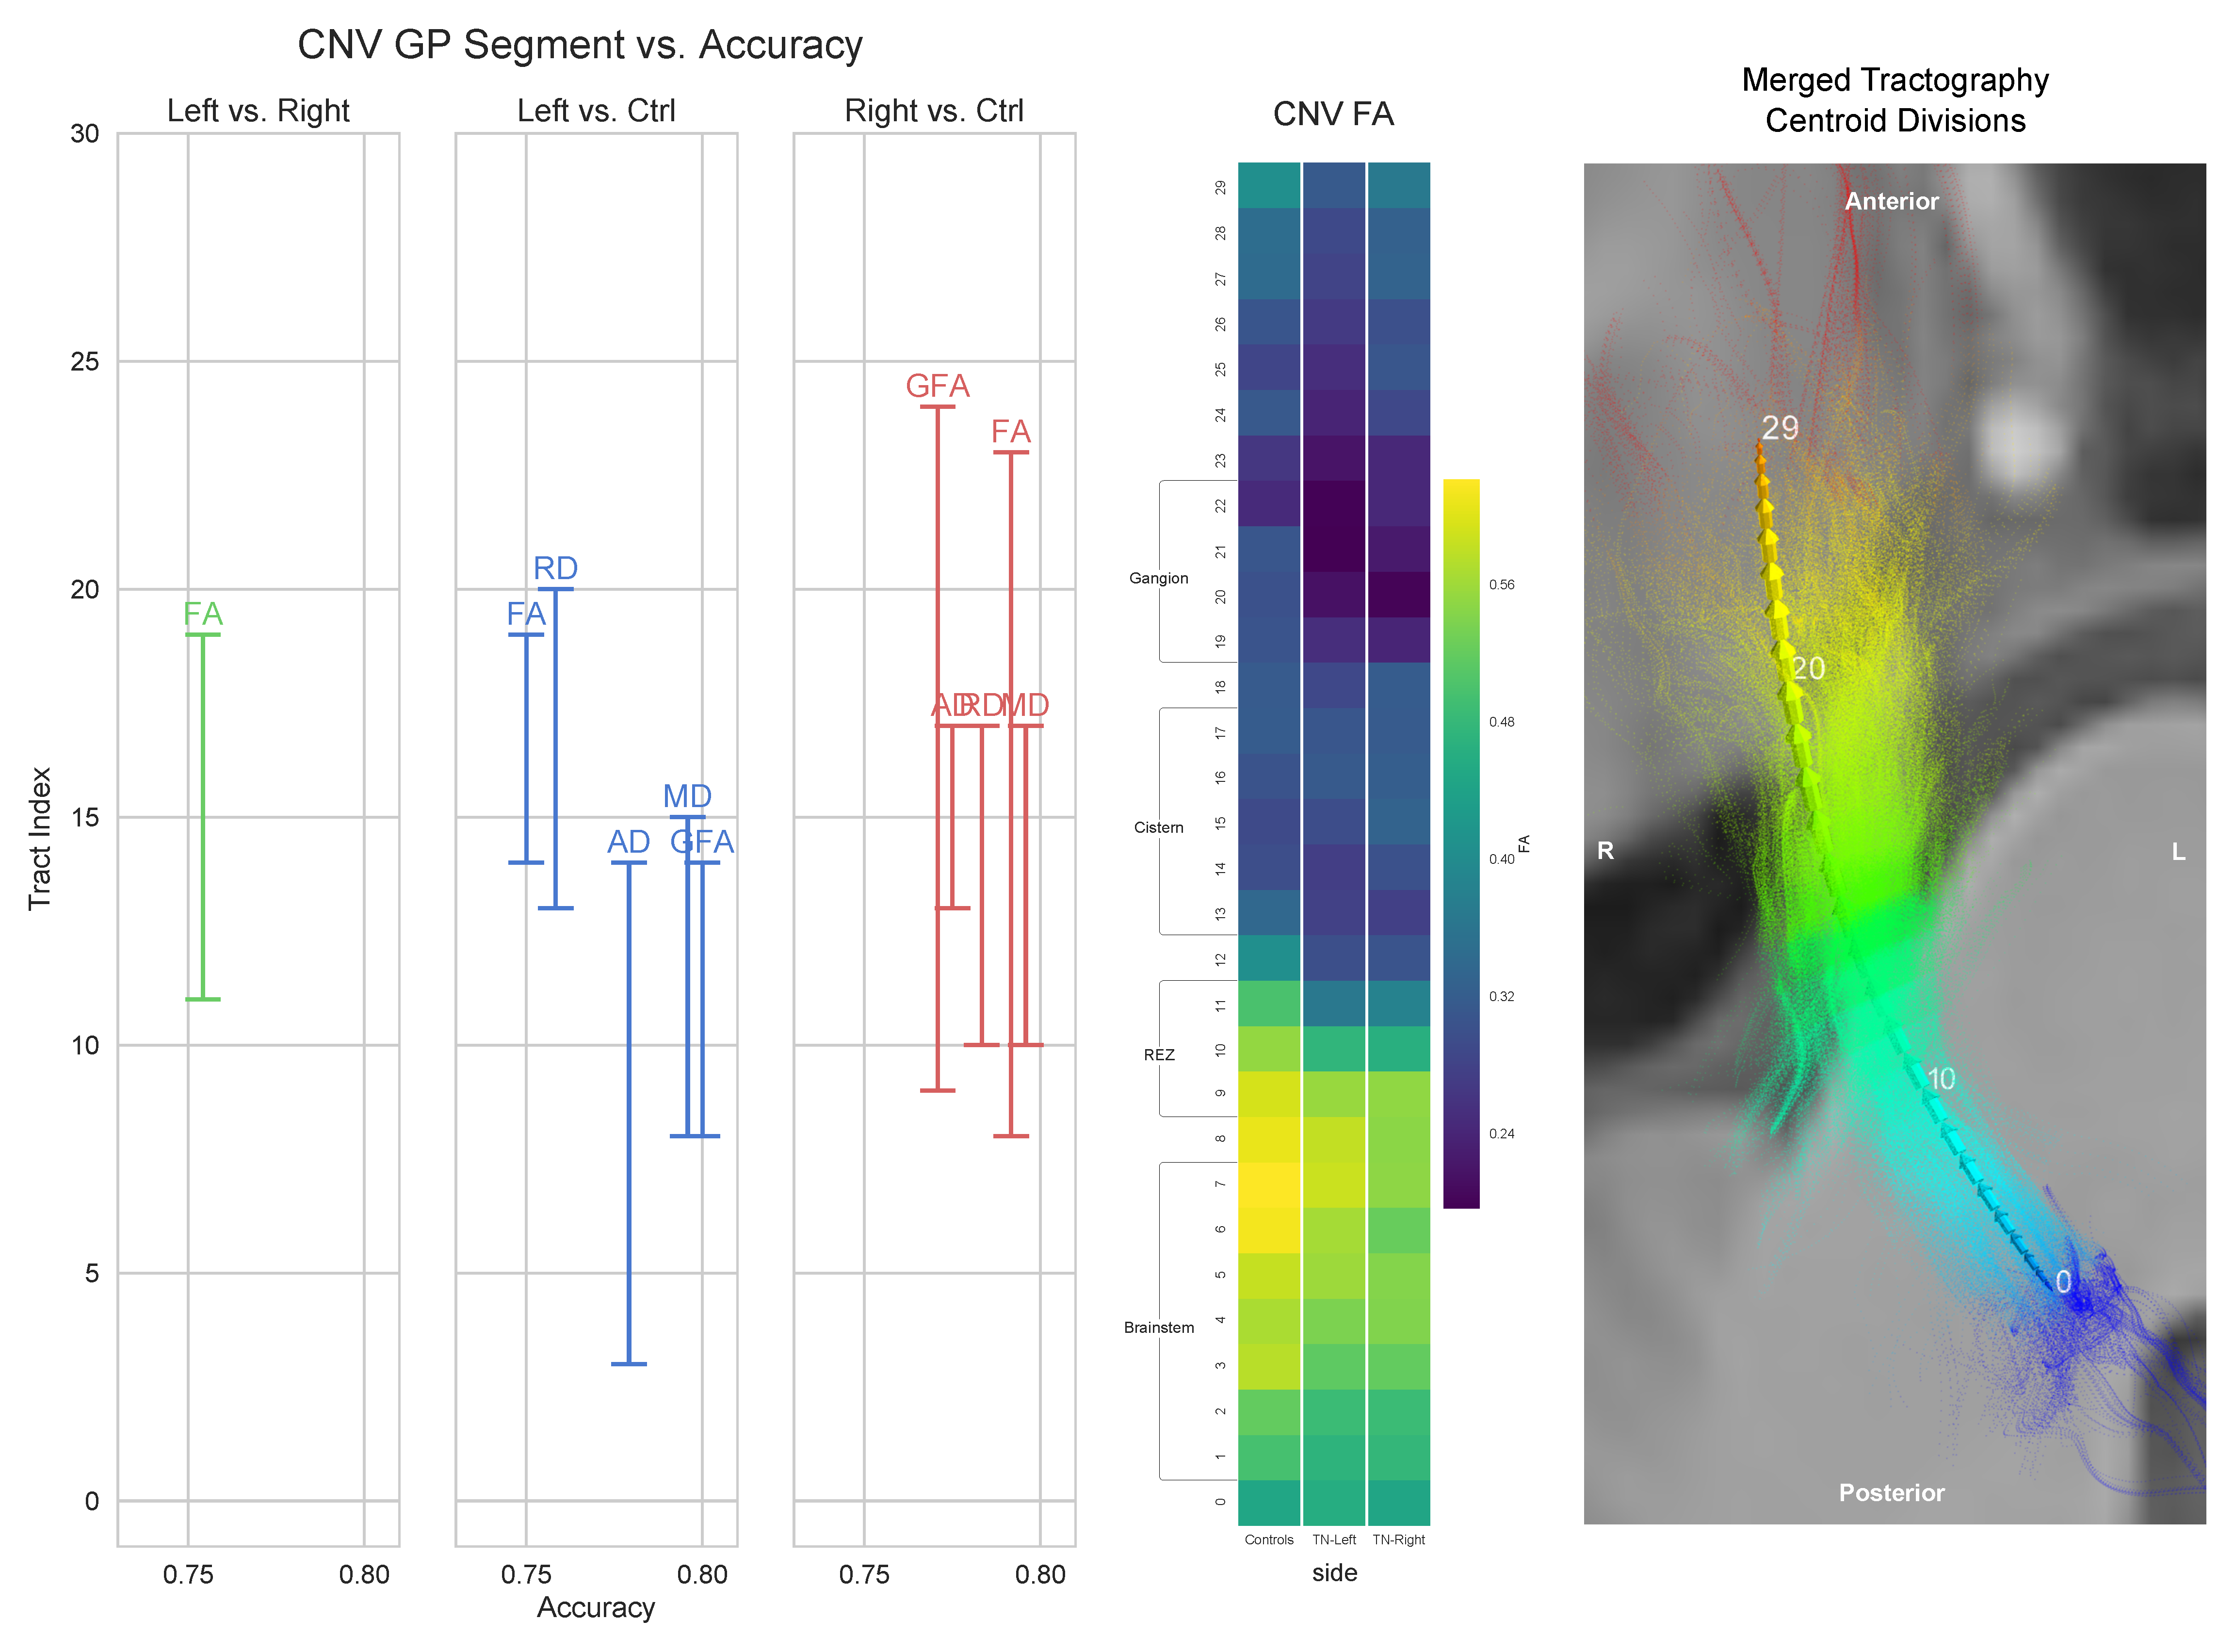
\includegraphics[width=\linewidth]{figure-GP-CNV.pdf}
\caption{CN V classifier performance}
\label{fig:GPfigure4}
\end{figure}

\begin{table}[ht]
\centering
\csvautotabular{cnv_table.csv}
\caption{CN V GP classifier performance data}
\caption*{List of the best accuracy for each diffusion metric. Precision, recall, and f1 scores are also provided for reference}
\label{table:CN V}
\end{table}

\paragraph{Trigeminopontothalamic tract}
Both left and right TPT pathways can be distinguished from controls with greater than 80\% accuracy (Figure \ref{fig:GPfigureTPT}). The right maximum accuracy was 85\% (FA), and minimum accuracy 83\% (RD), while the left maximum accuracy was 89\% (FA) and minimum 71\% (RD). The regions covered both the decussation and the ascending segments of the TPT, with the right decussation showing more proximal coverage. The left-right classifiers achieved maximum accuracy of 98\% (FA) and minimum of 88\% (MD). The left-right FA covered position 4--14, suggesting strong laterality differences in the TPT (Table \ref{table:tpt}). 

\begin{figure}[ht]
\centering
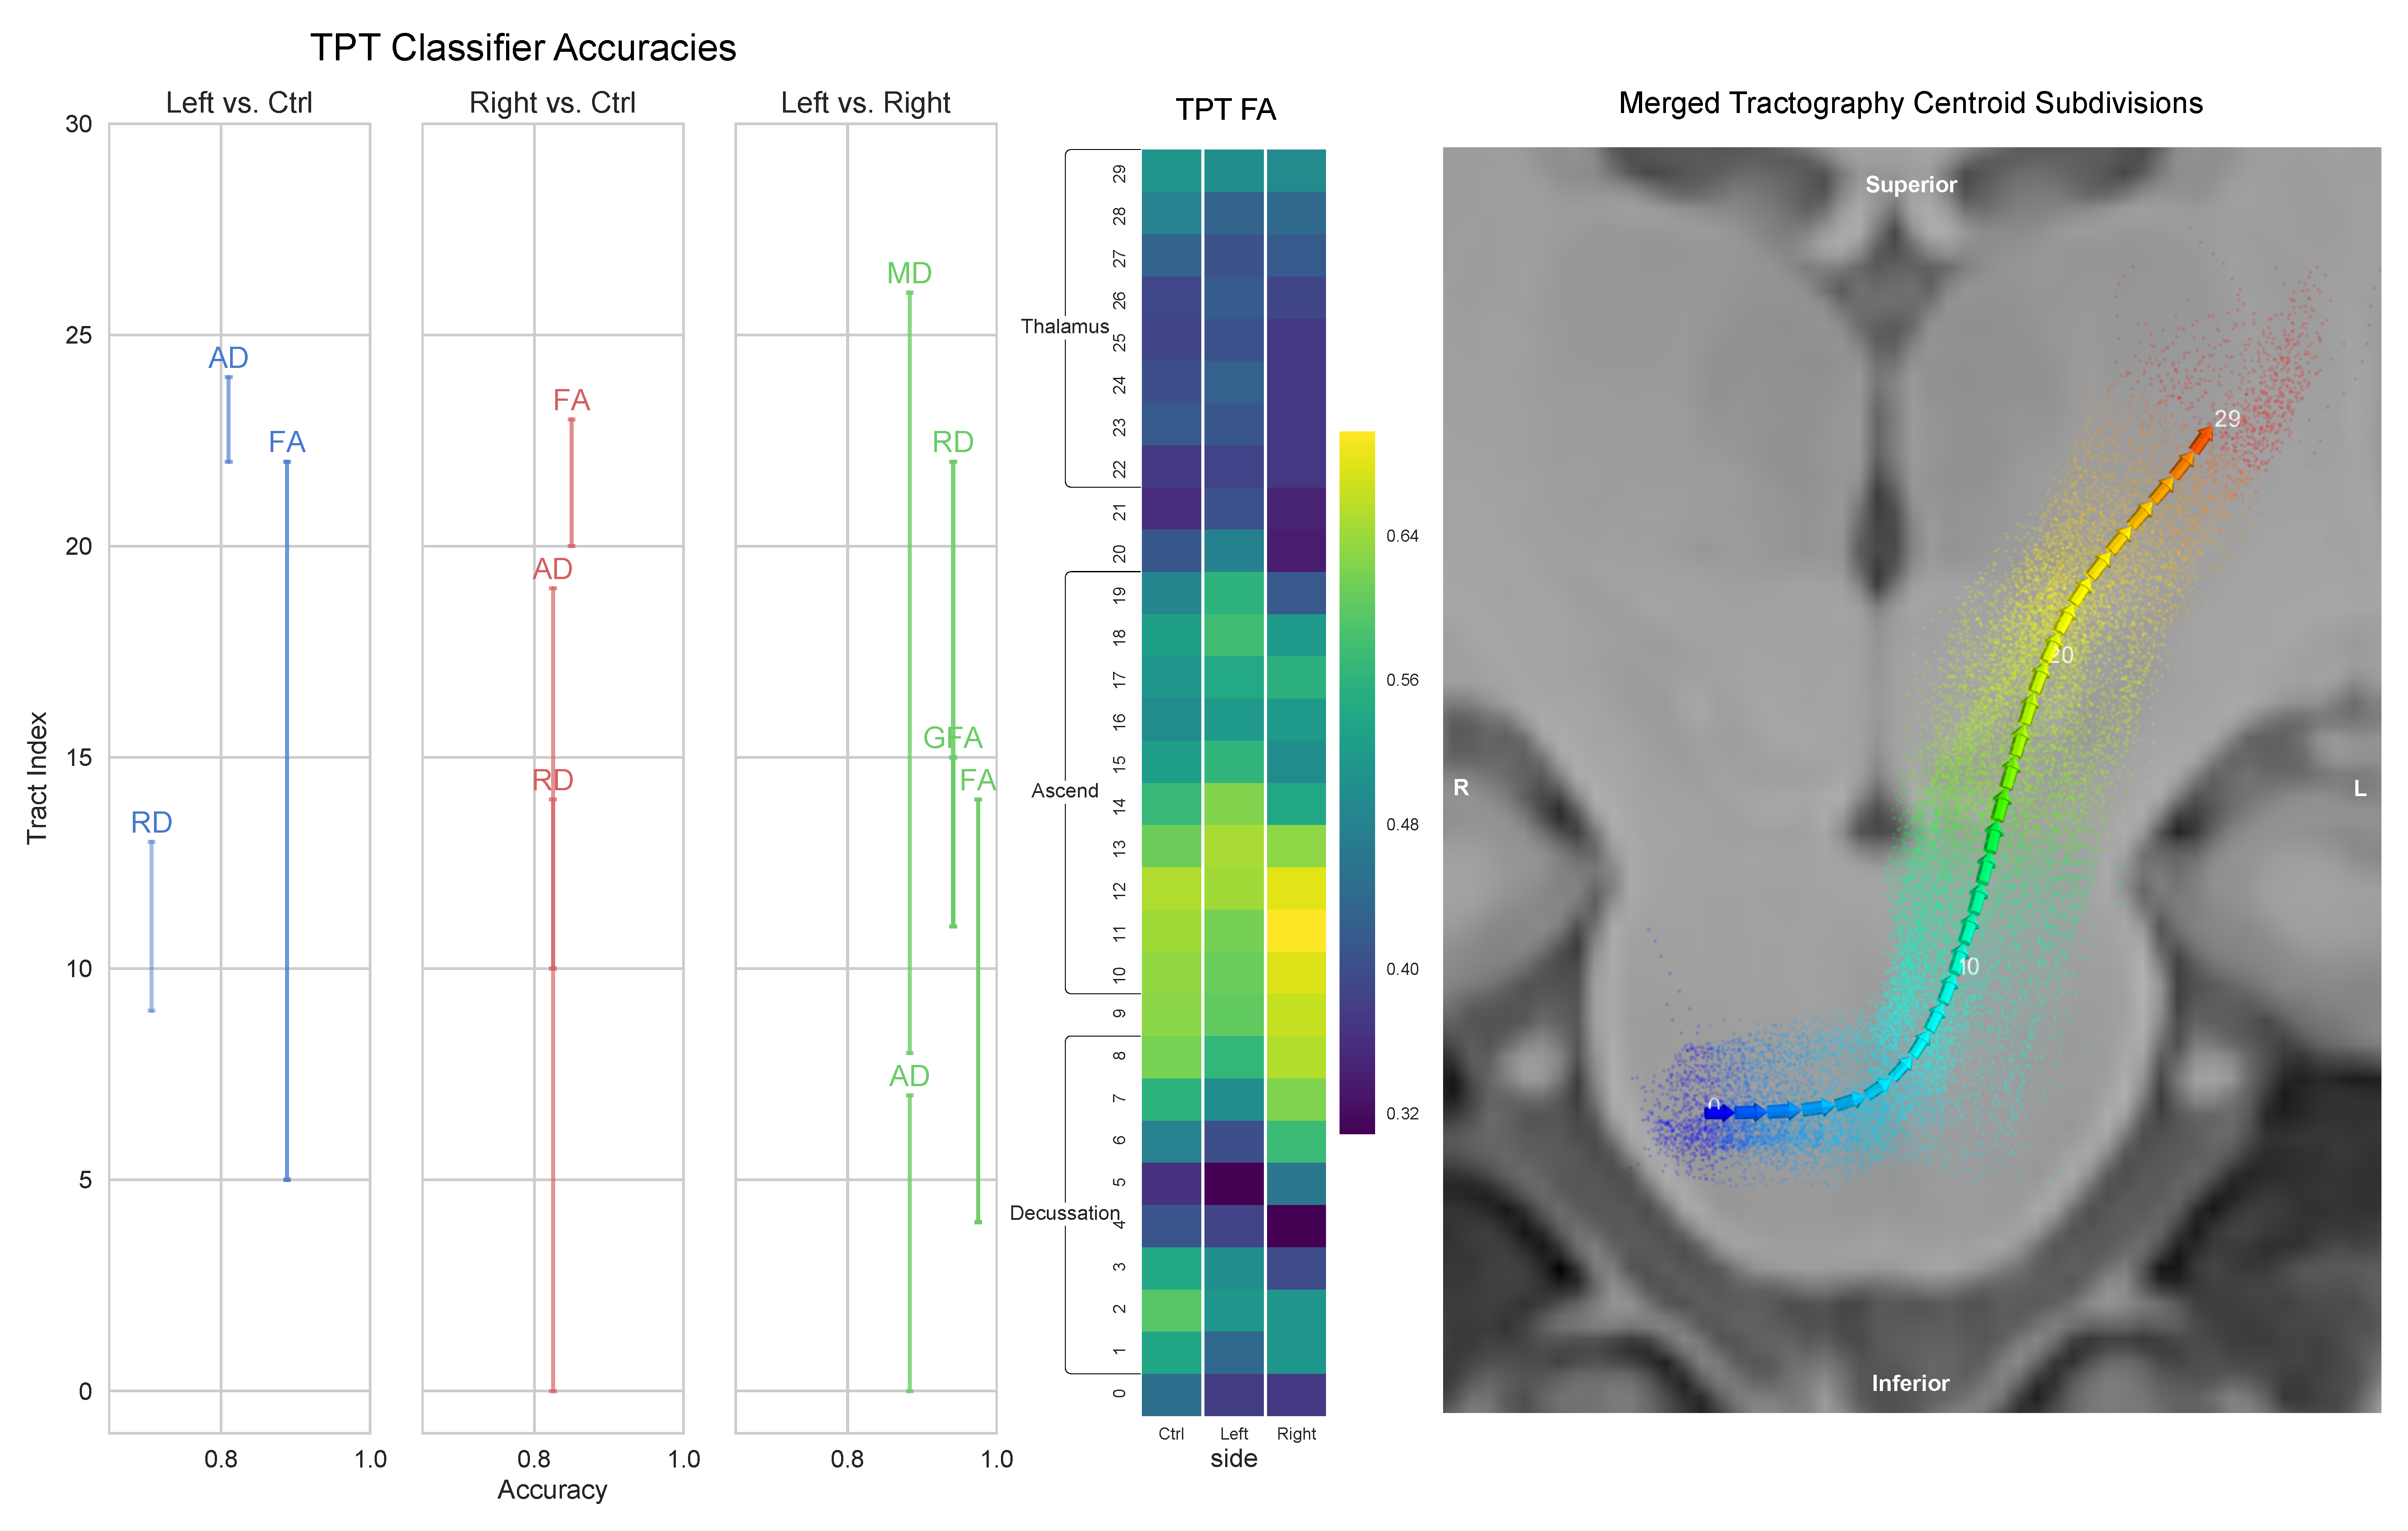
\includegraphics[width=\linewidth]{figure-GP-TPT.pdf}
\caption{TPT classifier performance}
\label{fig:GPfigureTPT}
\end{figure}

\begin{table}[ht]
\centering
\csvautotabular{tpt_table.csv}
\caption{TPT GP classifiers performance data}
\caption*{List of the best accuracies for each diffusion metric. Precision, recall, and f1 scores are also provided for reference}
\label{table:tpt}
\end{table}

\paragraph{S1}
Both sides of the S1 face region pathway were able to be distinguished by classifiers with about 85\% accuracy. The left RD classifier achieved max accuracy of 87\% at position 13--20, while the right RD classifier achieved max accuracy of 83\% at psotion 8--26 (Figure \ref{fig:GPfigure5}). Overall the left classifier ranged from 72\% (AD) to 87\% (RD), and the right classifieres ranged from 73\% (GFA) to 83\% (RD) (Table \ref{table:s1}). Both sides differ from controls in the branching region between the thalamus and cortex. Left-right classifiers showed maximum accuracy of 78\% (RD), and minimum of 76\% (FA). The left-right classifiers overlap in the regions 5--10, at the segment where the pathway emerges from the thalamus.

\begin{figure}[ht]
\centering
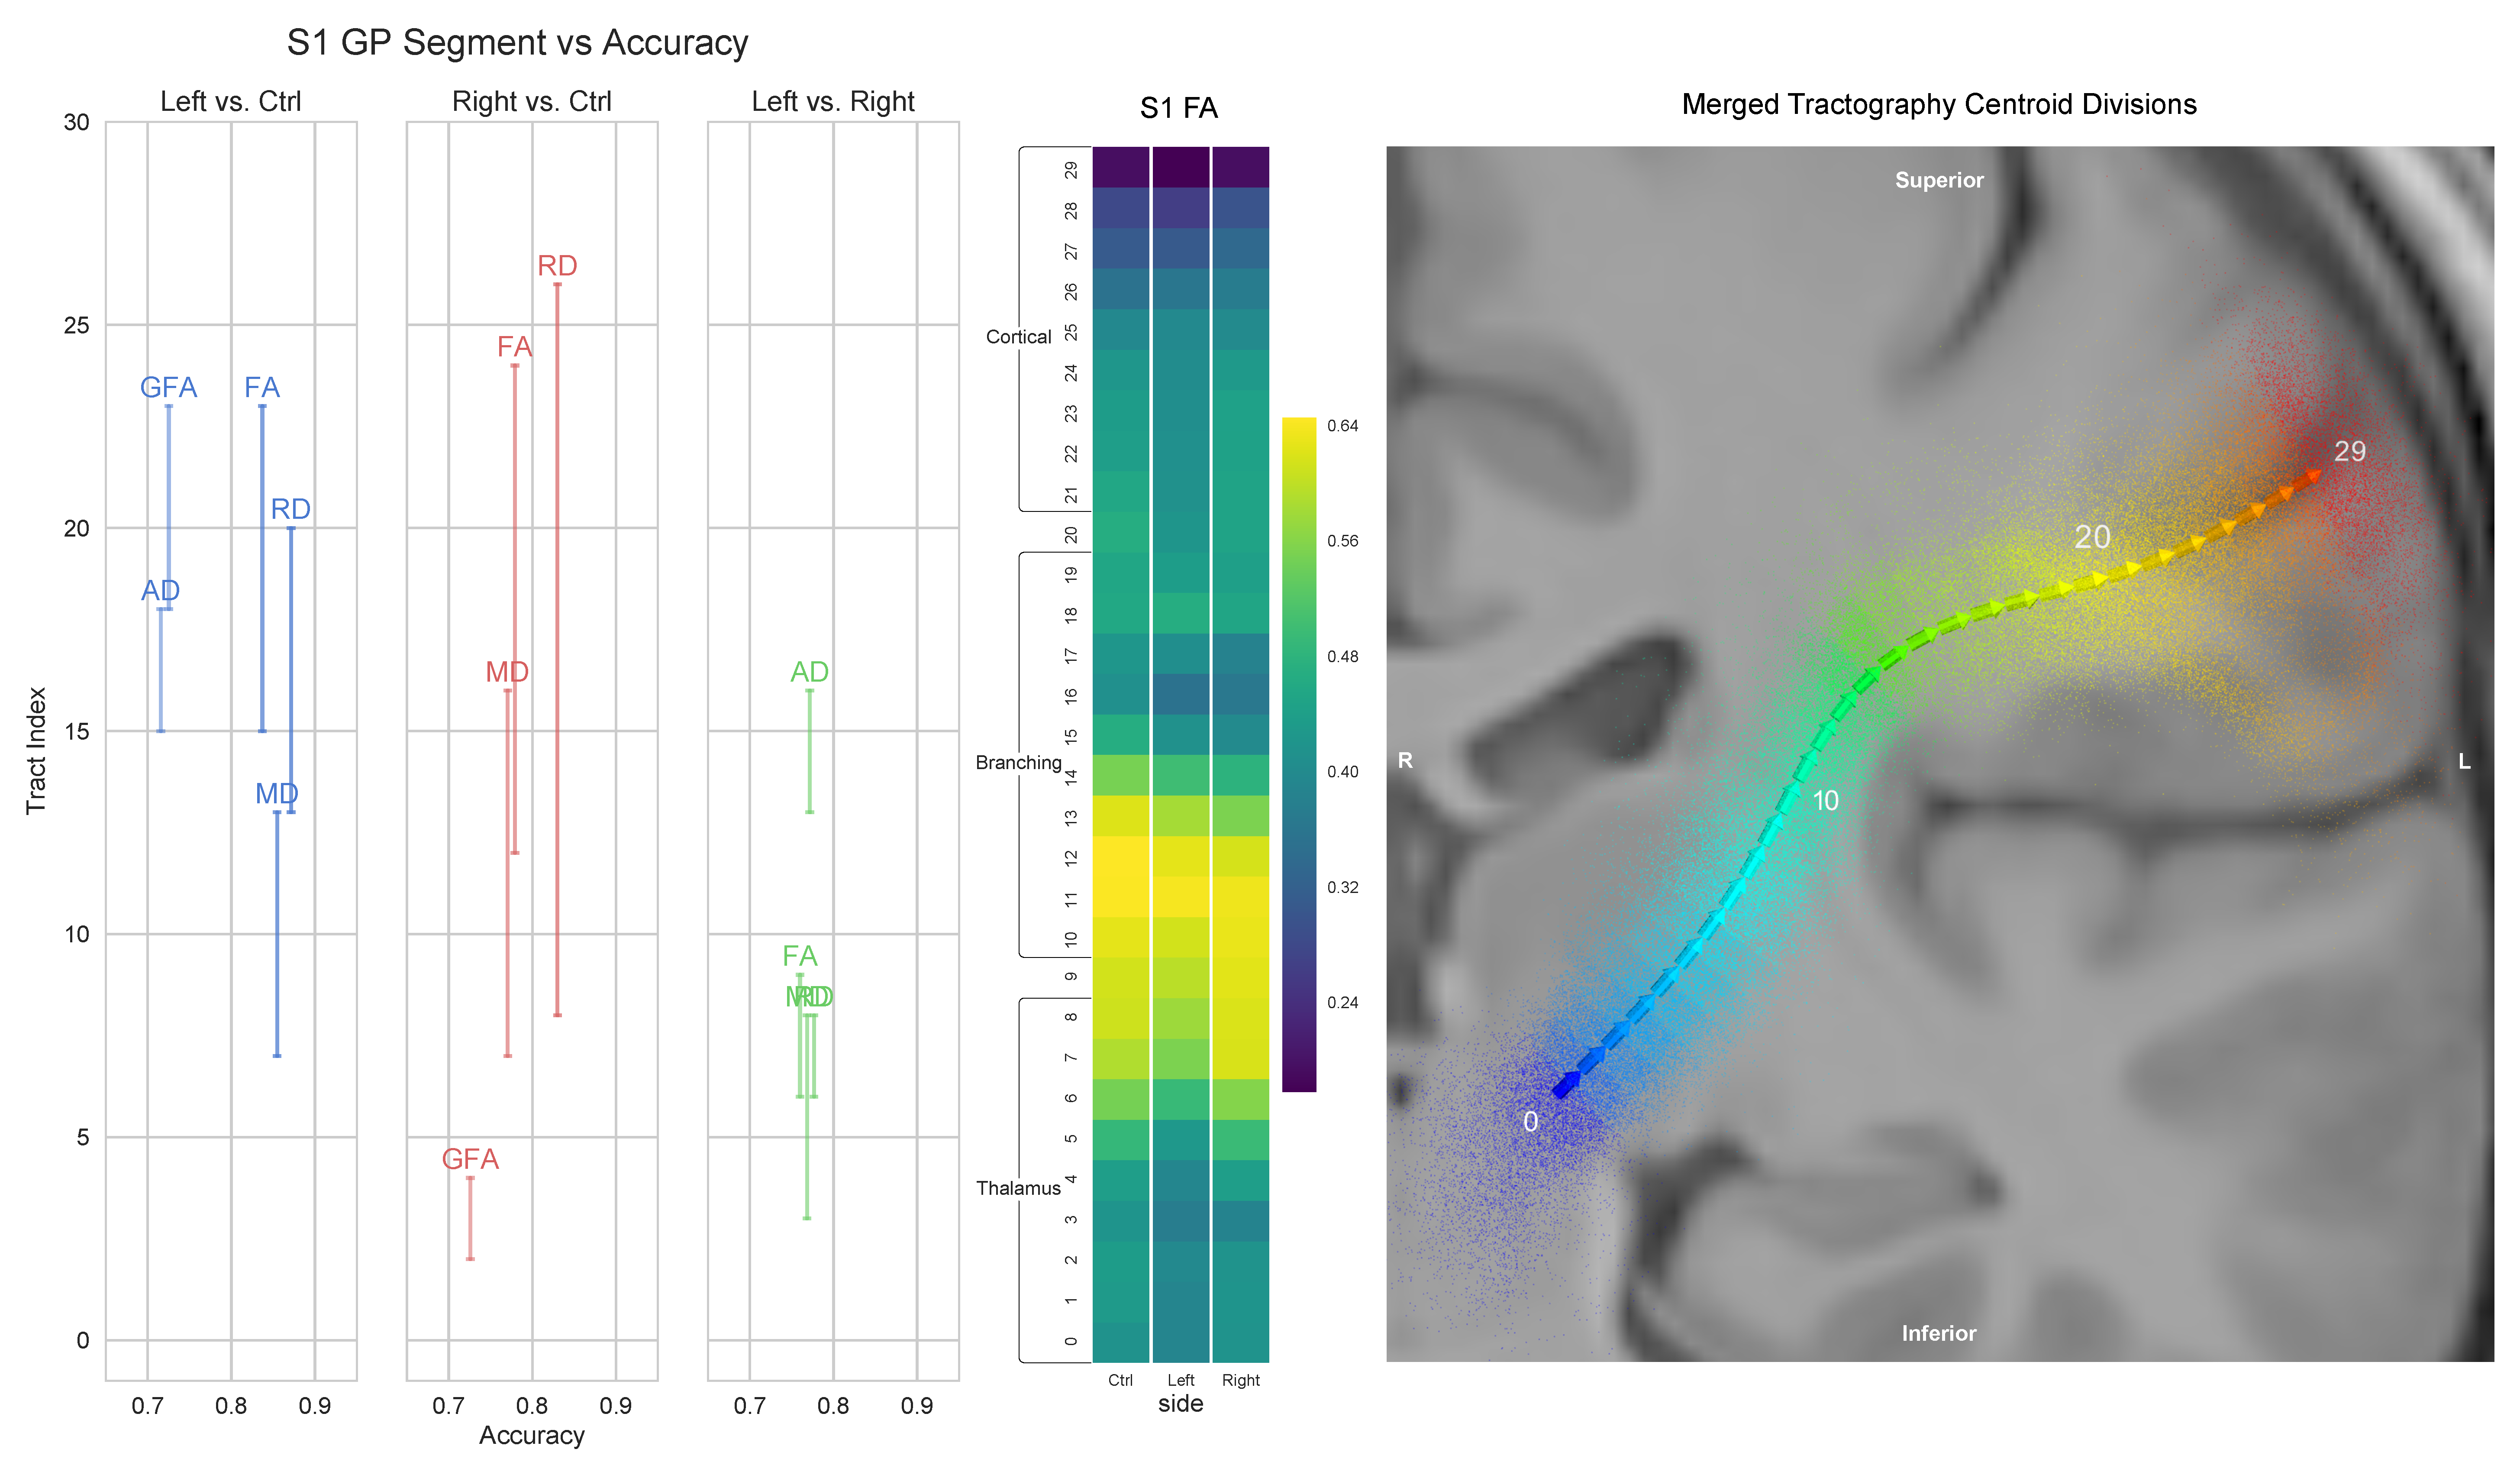
\includegraphics[width=\linewidth]{figure-GP-S1.pdf}
\caption{S1 classifier performance}
\label{fig:GPfigure5}
\end{figure}

\begin{table}[ht]
\centering
\csvautotabular{s1_table.csv}
\caption{S1 GP classifiers performance data}
\caption*{List of the best accuracies for each diffusion metric. Precision, recall, and f1 scores are also provided for reference}
\label{table:s1}
\end{table}

\section{Discussion}
The study is the first instance of machine learning discrimination of TN vs. Controls with specific white matter analysis, using group-wise merged along-the-track tractography. In essence, we have demonstrated a fully-automated, end-to-end tractography and machine learning platform that is capable of discriminate TN from white-matter diffusivity with greater than 80\% accuracy solely from white-matter measures. We reproduced previous findings of TN diffusivity changes along the CN V with much higher regional specificity. We also examined TPT and S1 projections of the trigeminal sensory pathway.

The diffusivity measures of CN V reproduced our previous findings \cite{Chen2016a}, which was that cistern, REZ differentiated TN from controls. The consistent regional overlaps in the cistern/ganglion region of the right (affected) CN V showed the ability for the GP classifiers to auto-converge to focal white-matter abnormality. The left versus right GP classifier placed left-right differences at the cistern/REZ segment, in agreement with the pathophysiology of TN. The regional findings on left versus controls suggest that there is bilateral differences in CN V myelin in unilateral TN, despite the lack of symptoms on the unaffected side. The left regions also situate into the brainstem segments. It is possible that the left CN V is affected by global descending pain modulation, and warrant further investigation. 

The TPT delineations showed that decussation pathway tractography is possibly asymmetric. It demonstrated very strong differences from the classifier results, with overlapping differences in the ascending segment. There also seemed to be diffusivity differences in the decussation segments between affected and unaffected sides. The decussaing fibers of the TPT emerges from the TGN, therefore the difference seemed reasonable. It is not clear however, whether the tractography asymmetry of the TPT is neuroanatomically factual, or an artifact from either algorithmic bias or partial volume bias of the underlying DWI. Resolving crossing fiber is still a difficult task in tractography, and while there are validations against MR phantoms, the anatomical validity of these methods can only be extrapolated, and the interpretation must involve anatomical priors from experts.  

The S1 delineation was consistent, due to full automation using SAGIT and the incorporation of Freesurfer cortical segmentation maps. Reproducing streamlines into the face-region of S1 cortex in multiple subjects was difficult previously due to individual variations, as well as the multi-directional fiber crossings in the coronal radiata. Previous studies have suggested that S1 have key involvement in pain location discrimination \cite{bushnell1999pain}, and are found to have grey-matter abnormalities in TN pain \cite{Desouza2013c}. Our finding that the left (affected) thalamocortical S1 projection is uniquely different close to the cortex suggest that deep cortical white-matter/grey-matter changes may be related depending on the locality. 

We included GFA to investigate its potential for measuring deep white-matter diffusivity, as it is the most well-known non-Gaussian diffusivity metric. However results demonstrated that it is not effective in pinpoint deep white-matter abnormalities. GFA did not perform to any substantially degree than the Gaussian-base diffusivity metrics. 

Overall the GP classifiers resulted in higher precision when compared to accuracy. The overlapping regions revealed differences in localizations that may very well have been missed with singular diffusivity metric analysis. This suggests that cross-metric features should be considered in future studies. This would drastically increase the feature complexity, and thereby require subsequent demand in the number of subjects. 

\subsubsection{Limitations}
The merged CN V delineations of all the subjects showed caudal projections towards the spinal cord. In multiple instances, diverging streamlines at the levels of the medulla strongly suggested the trigeminal spinal decussations. However the caudal projection was not available for the majority of the TN group, and it was not a consistently producible pathway. This is likely due to that 1) 3T DWI scan has a limited 2mm isovoxel resolution; It is not enough to resolve CN V, medullary and spinal cord fiber details. We have modified our scan to 1x1x3mm voxel, to gain axial plane detail for this kind of small fiber tractography from clinical scans, at the sacrifice of coronal/sagittal resolution. 2) A large percent of the TN DWI scans has severe distortions at the pontine level. Similar distortions rarely show up in Control or MS-TN scans. The reason may be due to the changes in the vertebral and basilar blood vessels that gave rise to EPI distortions in these patients. These distortions narrow the brainstem in the DWI image, and when combined with limited resolution, making tractography delineations even more difficult. Therefore, it is highly recommended to perform reverse-blip DWI acquisitions in patients with cerebral vessel irregularities as part of MR DWI clinical practice. 

The diffusivity metrics of the deeper white matter structures remains difficult to interpret, due to the complex crossing fibers in these regions. Although metrics such as FA are popular in current neuroimaging literature, they nevertheless are derived from the Gaussian tensor model, which cannot adequately describe cross-fiber regional dynamics. For example, in the crossing-fiber region of healthy tissue, where both bundles have equal myelin and axonal integrity, will have a low FA score due to a spherical tensor; its AD and RD will be roughly equal, and therefore MD will be higher. In a pathological cross region, where only one bundle is healthy, the FA increases due to the diffusivity bias in one direction; the RD will be lower, and MD will be lower as well. Moreover, in diverging and converging structures, as well as in multi-crossing regions such as the corona radiata, the interpretations of Gaussian-based diffusivity metrics become even more unclear. Therefore, it is imperative that interpretable diffusivity measures for crossing regions be established and adopted by the neuroimaging tractography field for future studies. 

\subsection{Conclusions}
We have demonstrated the first instance of group-wise merged along-the-track tractography analysis of TN vs. control. We have achieved examination of specific and targeted anatomy at a group level involving both healthy and pathological brain images. The method reproduced previous findings of TN diffusivity changes along the CN V with finer-grained regional specificity. We also examined TPT and S1 projections of the trigeminal sensory pathway. The study revealed that there are specific diffusivity changes on these deeper white matter structures, and demonstrated the power of along-the-tract analysis with machine-learning, which pinpoints the exact location of the diffusivity disruption at millimetre level. 
